% !TEX root = ../zenkoku.tex
\section{結果?}

理解度は値が高いほど理解が深いものとし,`熟練者の理解度 - 熟練者を除いた回答者の理解度平均` によって求めた数値を熟練者への依存度の高さとする.
結果を\ri{img:rikai}に示す.

この辺から分析

% memo: これは結果より後
%分析フェーズで熟練した開発者がチームに1人いる状況を想定し,この開発者への依存度が高いようなシステムを洗い出すことにした.



属人性の高さとしてはシステムAやシステムBのフロントエンド領域などにおいて熟練者への依存度の高さが(TODO:ここに強調の語彙)だが,システムGのように差が0.4ポイントしか見られないようなものもある.
またシステムKやシステムHのバックエンド領域など熟練者,平均ともに理解度の低いものも見受けられ,これは開発組織内で誰も詳細を知らないシステムとなっていると考えられる.

この結果を開発組織内に対し討論する機会を設けたところ以下のような意見が出た.

% ここの書き方考え中
- 小規模なチームではトラック係数を上げないとチームメンバーの退職とかで立ち行かなくなることがありえる
- 熟練者への依存度を下げたい という思いはあるが何から始めたらいいかわからない状況がある. good First issue とかを用意してはどうか
- 出てきた理解度の平均,熟練者への依存度共に大きな認識の相違はなさそう


\begin{figure}
	\centering
	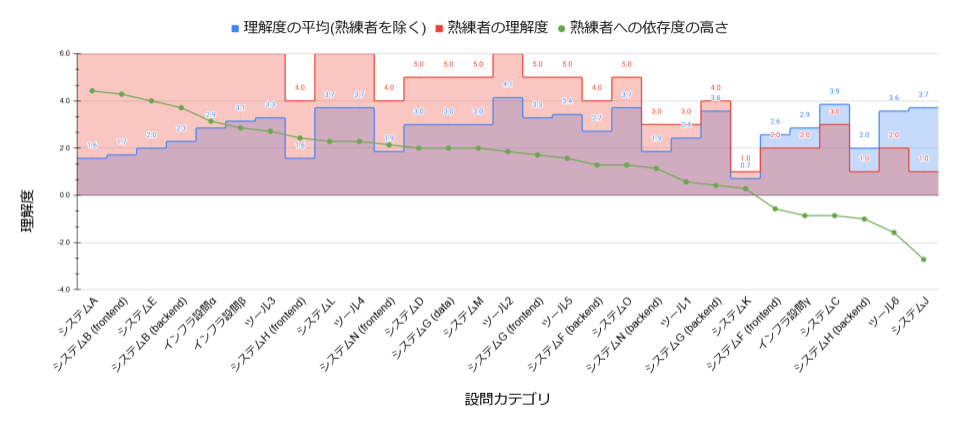
\includegraphics[keepaspectratio,width=0.9\linewidth]{img/rikai.png}
	\caption{理解度の平均と熟練者への依存度の高さ}
	\label{img:rikai}
\end{figure}
